%%% Класс документа
\documentclass[a4paper,14pt]{article}

%%% Работа с русским языком
\usepackage{cmap}					% поиск в PDF
\usepackage[warn]{mathtext}
\usepackage[T2A]{fontenc}			% кодировка
\usepackage[utf8]{inputenc}			% кодировка исходного текста
\usepackage[english,russian]{babel}	% локализация и переносы
\usepackage{mathtext} 				% русские буквы в формулах
\usepackage{csvsimple}              % for tabular from csv loading
\usepackage{indentfirst}            % indent after sections
%\usepackage{minipage}

%%% Дополнительная работа с математикой
\usepackage{amsmath,amsfonts,amssymb,amsthm,mathtools} % AMS
\usepackage{icomma} % "Умная" запятая: $0,2$ --- число, $0, 2$ --- перечисление

%%% Номера формул
%\mathtoolsset{showonlyrefs=true} % Показывать номера только у тех формул, на которые есть \eqref{} в тексте.
%\usepackage{leqno} % Немуреация формул слева

%%% Шрифты
\usepackage{euscript}	 % Шрифт Евклид
\usepackage{mathrsfs} % Красивый матшрифт

%%% Свои команды
\DeclareMathOperator{\sgn}{\mathop{sgn}}

%%% Перенос знаков в формулах (по Львовскому)
\newcommand*{\hm}[1]{#1\nobreak\discretionary{}
{\hbox{$\mathsurround=0pt #1$}}{}}

%%% Работа с картинками
\usepackage{graphicx}  % Для вставки рисунков
\graphicspath{{images/}{images2/}}  % папки с картинками
\setlength\fboxsep{3pt} % Отступ рамки \fbox{} от рисунка
\setlength\fboxrule{1pt} % Толщина линий рамки \fbox{}
\usepackage{wrapfig} % Обтекание рисунков и таблиц текстом

%%% Работа с таблицами
\usepackage{array,tabularx,tabulary,booktabs} % Дополнительная работа с таблицами
\usepackage{longtable}  % Длинные таблицы
\usepackage{multirow} % Слияние строк в таблице

%%% Теоремы
\theoremstyle{plain} % Это стиль по умолчанию, его можно не переопределять.
%\newtheorem{theorem}{Теорема}[section]
%\newtheorem{proposition}[theorem]{Утверждение}
 
%\theoremstyle{definition} % "Определение"
%\newtheorem{corollary}{Следствие}[theorem]
%\newtheorem{problem}{Задача}[section]
 
%\theoremstyle{remark} % "Примечание"
%\newtheorem*{nonum}{Решение}

%%% Программирование
\usepackage{etoolbox} % логические операторы

%%% Страница
\usepackage{extsizes} % Возможность сделать 14-й шрифт
\usepackage{geometry} % Простой способ задавать поля
	\geometry{top=25mm}
	\geometry{bottom=35mm}
	\geometry{left=35mm}
	\geometry{right=20mm}
	
%%% Колонтитулы
%\usepackage{fancyhdr}
 	%\pagestyle{fancy}
 	%\renewcommand{\headrulewidth}{0mm}  % Толщина линейки, отчеркивающей верхний колонтитул
 	%\lfoot{Нижний левый}
 	%\rfoot{Нижний правый}
 	%\rhead{Верхний правый}
 	%\chead{Верхний в центре}
 	%\lhead{Верхний левый}
 	% \cfoot{Нижний в центре} % По умолчанию здесь номер страницы
 	
%%% Интерлиньяж
%\usepackage{setspace}
%\onehalfspacing % Интерлиньяж 1.5
%\doublespacing % Интерлиньяж 2
%\singlespacing % Интерлиньяж 1

%%% Гиперссылки
\usepackage{hyperref}
\usepackage[usenames,dvipsnames,svgnames,table,rgb]{xcolor}
\hypersetup{				% Гиперссылки
    unicode=true,           % русские буквы в раздела PDF
    pdftitle={Заголовок},   % Заголовок
    pdfauthor={Автор},      % Автор
    pdfsubject={Тема},      % Тема
    pdfcreator={Создатель}, % Создатель
    pdfproducer={Производитель}, % Производитель
    pdfkeywords={keyword1} {key2} {key3}, % Ключевые слова
    colorlinks=true,       	% false: ссылки в рамках; true: цветные ссылки
    linkcolor=red,          % внутренние ссылки
    citecolor=green,        % на библиографию
    filecolor=magenta,      % на файлы
    urlcolor=cyan           % на URL
}

%%% Другие пакеты
\usepackage{lastpage} % Узнать, сколько всего страниц в документе.
\usepackage{soul} % Модификаторы начертания
\usepackage{csquotes} % Еще инструменты для ссылок
%\usepackage[style=authoryear,maxcitenames=2,backend=biber,sorting=nty]{biblatex}
\usepackage{multicol} % Несколько колонок
\usepackage{multirow} % Несколько строк

%%% Шрифты
%\renewcommand{\familydefault}{\sfdefault} % Начертание шрифта


%%% Работа с библиографией
%\usepackage{cite} % Работа с библиографией
%\usepackage[superscript]{cite} % Ссылки в верхних индексах
%\usepackage[nocompress]{cite} % 
%\usepackage{csquotes} % Еще инструменты для ссылок


%%% Tikz
\usepackage{tikz} % Работа с графикой
\usepackage{pgfplots} % Работа с pgf
\usepackage{pgfplotstable}
\usepackage{upgreek}

%%% Дополнительные пакеты для tikz
%\usepgfplotslibrary{dateplot} % Возможность подписания дат
\pgfplotsset{compat=1.5}

\begin{document}
	\newcommand{\HRule}{\rule{\linewidth}{0.7mm}} % Defines a new command for the horizontal lines, change thickness here
	
	\begin{center}
		\large\textbf{Московский Физико-Технический Институт}\\ % Name of your university/college
		\large\textbf{(государственный университет)}
	
		\vfill
		
		\Large Лабораторная работа по курсу общей физики № *labnum*\\[0.5cm] % Preambule of your document title
		
		
		\HRule
		\\[0.4cm]
		{ \huge \bfseries *name of your labwork*}% Title of your document
		\\[0.4cm] 
		\HRule
		\\[0.5cm]
		
		\ \\
	\textbf{\large Автор:} \\	
	\large *your name* *groupname*\\ % Your name and something more, your group num for example
		\vfill
		\hspace*{-0.8 cm}
\includegraphics[width=100 pt]{frkt_logo}\\ % logo of your  company/university/college
		\large Долгопрудный, 2021 % location and year
	\end{center}

\newpage
\setcounter{page}{2}
\fancyfoot[c]{\thepage}
\fancyhead[L] {Работа № *labnum*} % some information in page header
\fancyhead[R]{}
	
	\section*{Задание 1.}
	
	\noindent Соберем на макетной плате схему интегрирующей цепи с параметрами $R = 100$ Ом, $C = 1,05$ мкФ, тогда постоянная времени для этой цепи $\tau = R C = 105$ мкс.
	
	\noindent Экспериментально определим верхнюю граничную частоту $\nu_0$, подбирая $\nu_0$ таким образом, чтобы амплитуда выходного сигнала составила $70 \%$ от амплитуды входного сигнала. $U_{\text{вых}} = 0,7 U_{\text{вх}}$.
	
	\noindent Теоретическое значение $\nu_{\text{0теор}} = \frac{1}{2 \pi C R} = 1,516$ кГц. Экспериментальное значение $\nu_{\text{0экс}} = 1,51$ кГц.
	
	%---------------------------------------------------------------------------------------------------------------------------------------------------------------
	
	\noindent Снимем зависимость коэффициента передачи $K(\nu) = \frac{U_{\text{вых}}}{U_{\text{вх}}}$ от частоты $\nu = 2^n \nu_0$ в пределах $n \in [-2, 4]$. Построим график $K(\nu)$, а так же граф Боде -- $20 \lg K$ от $n = \log_2 (\nu / \nu_0)$.

	\begin{table}[h!]
		\begin{center}
			\begin{tabular}{|c|c|c|c|}
				\hline
				$n$& $\nu$, кГц & $K(\nu)$ &  $20 \lg K$      \\ \hline
				-2 & 0,377      & 0,96     & -0,35  \\ \hline
				-1 & 0,755      & 0,9      & -0,92  \\ \hline
				0  & 1,51       & 0,73     & -2,73  \\ \hline
				1  & 3,02       & 0,55     & -5,19  \\ \hline
				2  & 6          & 0,32     & -9,90  \\ \hline
				3  & 12         & 0,16     & -15,92 \\ \hline
				4  & 24,1       & 0,088    & -21,11 \\ \hline
			\end{tabular}
		\end{center}
		\caption{}
	\end{table}

	% график 1
	% график 2
	% картинка колебаний
	
	%---------------------------------------------------------------------------------------------------------------------------------------------------------------
	
	\noindent По осцилограмме прямоугольных сигналов оценим постоянную времени $\tau$,\\ измерив время нарастания фронта импульса от нуля до уровня $1 - 1/e \approx 0,63$.
	
	\noindent Экспериментально получено $\tau = 111$ мкс. Тогда $\nu_0 = \frac{1}{2 \pi \tau} \approx 1434$ Гц.
	
	% картинка прямоугольных сигналов. 
	
	%---------------------------------------------------------------------------------------------------------------------------------------------------------------
	
	\noindent Соберем на макетной плате схема интегрирующей цепи. Экспериментально определим нижнюю граничную частоту $\nu_0$.
	
	\noindent Теоретическое значение $\nu_{\text{0теор}} = \frac{1}{2 \pi C R} = 1,516$ кГц. Экспериментальное значение $\nu_{\text{0экс}} = 1,9$ кГц.
	
	%---------------------------------------------------------------------------------------------------------------------------------------------------------------
	
	\noindent Снимем зависимость коэффициента передачи $K(\nu) = \frac{U_{\text{вых}}}{U_{\text{вх}}}$ от частоты $\nu = 2^n \nu_0$ в пределах $n \in [-4, 2]$. Построим график $K(\nu)$, а так же граф Боде -- $20 \lg K$ от$n = \log_2 (\nu / \nu_0)$.
	
	
	\begin{table}[h!]
		\begin{center}
			\begin{tabular}{|c|c|c|c|}
				\hline
				n  & $\nu$, Гц & $K(\nu)$ & $20 \lg K$  \\ \hline
				-4 & 118,7     & 0,07     & -23,10 \\ \hline
				-3 & 237,5     & 0,11     & -19,17 \\ \hline
				-2 & 475       & 0,246    & -12,18 \\ \hline
				-1 & 950       & 0,43     & -7,33  \\ \hline
				0  & 1900      & 0,69     & -3,22  \\ \hline
				1  & 3800      & 0,87     & -1,21  \\ \hline
				2  & 7600      & 0,95     & -0,45  \\ \hline
			\end{tabular}
		\end{center}
		\caption{}
	\end{table}
	
	% график 1
	% график 2
	% картинка колебаний

	%---------------------------------------------------------------------------------------------------------------------------------------------------------------

	\noindent Изучим графики частотной и фазовой характеристик интегрирующей цепи в MicroCap. 
	Верхняя частота $f_0 = 9,99 \approx 10$ кГц. Изучим переходную характеристику.

	\noindent Расчитаем постоянную времени $\tau = (R || R_L) \cdot C = 16$ мкс, значение, найденное по графику $\tau = 16,5$ мкс.

	\noindent Убедимся в том, что при наличии сопротивления $R_L$ передаточная функция
	цепи принимает вид

	\begin{equation*}
		H(p) = \frac{K_0}{1 + p \tau}, ~ K_0 = \frac{R_L}{R + R_L}, ~ \tau = (R || R_L) \cdot C
	\end{equation*}

	\begin{figure}[h!]
		\centering
		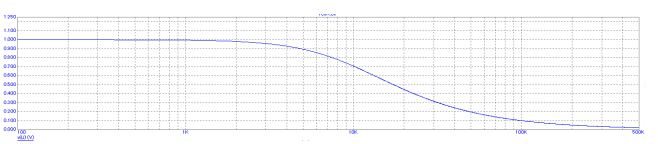
\includegraphics[scale = 0.7]{MC_task1.1.png}
		\caption{}
	\end{figure}

	%-------------------------------------------------------------------------------------------------------------------------

	\noindent Изучим частотную и фазовую характеристики дифференцирующей цепи. Нижняя частота $f_0 \approx 10$ кГц. Изучим переходную
	характеристику. По графику оценим постоянную времени $\tau \approx 16,9$ мкс. 
	Убедимся, что при $R_s \neq 0$ передаточная функция принимает вид

	\begin{equation*}
		H(p) = \frac{K_0 p \tau}{1 + p \tau}, ~ K_0 = \frac{R}{R + R_s}, \tau = (R + R_s) \cdot C
	\end{equation*}

	\begin{figure}[h!]
		\centering
		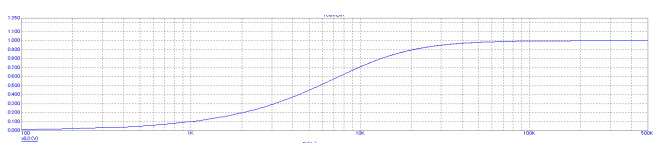
\includegraphics[scale = 0.7]{MC_task1.2.png}
		\caption{}
	\end{figure}	

	% =======================================================================================================================
	
	\section*{Задание 2.}

	\begin{equation*}
		f_0 = \frac{1}{2 \pi RC} = 10 ~ \text{кГц}
	\end{equation*}

	\noindent По графикам ФЧХ измерим значения фазовых
	сдвигов ФВЧ, ПФ и ФНЧ на частотах $0, ~ f_0, ~ \infty$.

	\begin{table}[h!]
		\begin{center}
			\begin{tabular}{|c|c|c|c|}
				\hline
							& ФВЧ & ПФ  & ФНЧ0 \\ \hline
				0       	& 180 & 90  & 0    \\ \hline
				$f_0$   	& 90  & 0   & -90  \\ \hline
				$\infty$	& 0   & -90 & -180 \\ \hline
			\end{tabular}
		\end{center}
	\end{table}

	\noindent Заметим, что двухсторонняя полоса пропускания ПФ $\Delta f = 36 - 3 ~ \text{кГц} = 33 ~ \text{кГц} \approx 3f_0$ .

	%-------------------------------------------------------------------------------------------------------------------------

	Открыв графики переходных характеристик, оценим время спада $\tau^{(-)}$ первого выброса
	переходной характеристики ФВЧ до уровня $e^{-1}$ и время $\tau^{(+)}$ нарастания фронта переходной
	характеристики ФНЧ до уровня $1 - e^{-1}$.

	\begin{center}
		\fbox{$\tau^{(-)} = 4,3 ~ \text{мкс} ~~ \tau^{(+)} = 53,0 ~ \text{мкс}$}
	\end{center}

	\begin{center}
		\fbox{$\frac{\tau^{(+)}}{\tau^{(-)}} = 12,24$}
	\end{center}

	% =======================================================================================================================

	\section*{Задание 3.}

	\noindent Наибольший диапазон перестройки фазы реализуется на частоте $f_0 = 25$ кГц. При этом, границы этого диапазона
	$[-150, 73^o, -28,73^o]$.
	
	%------------------------------------------------------------------------------------------------------------------------

	\noindent Изучим частотную и фазовую характеристики двойного Т-образного моста. 
	\noindent Ширина полосы реженции $\Delta f = 41, 18 - 2,38 \approx 39 ~ \text{кГц} ~ \approx 4 F_0$.

	%------------------------------------------------------------------------------------------------------------------------

	\noindent Подключим ко входу источник прямоугольного импульса и проанализируем переходную характеристику. 
	Оценим время спада $\tau^{(-)} = 4,2$ мкс и нарастание $\tau^{(+)} = 67 - 12 = 55$ мкс.
	\noindent Теоретические значения

	\begin{equation*}
		\tau^{(\pm)} = \frac{1}{2 \pi f_0 \mu_{\pm}}, ~ \mu_{\pm} = 2 \pm \sqrt{3}
	\end{equation*}

	%------------------------------------------------------------------------------------------------------------------------

	\noindent Оценим частоты $f_0$ и добротность $Q = \frac{f_0}{\Delta f}$ нулей передачи.

	\begin{table}[h!]
		\begin{center}
			\begin{tabular}{|c|c|c|c|}
				\hline
				$R$, кОм & $f_0, кГц$ & $\Delta f$, Гц  & $Q$      \\ \hline
				4,9      & 9,94       & 100             & 99       \\ \hline
				5,0      & 10,00      & 1               & 10000    \\ \hline
				5,1      & 10,05      & 98              & 103      \\ \hline
			\end{tabular}
		\end{center}
	\end{table}

	\noindent Групповые задержки

	\begin{center}
		$R = 4,9$ кГц, $f = 10,05$ кГц | $\tau_g = 3$ мс, $\tau_{теор} = \frac{Q}{\pi f} = $ \\
		$R = 5,1$ кГц, $f = 9,95$  кГц | $\tau_g = 3$ мс, $\tau_{теор} = \frac{Q}{\pi f} = $
	\end{center}

	% ========================================================================================================================
	\section*{Задание 4.}

	\noindent Параметры компонентов.

	\begin{center}
		$L = 220$ мкГн \\
		$R = 91$  Ом   \\
		$C = 1,2$ нФ   \\
	\end{center}

	\noindent На макетной плате соберём схему полосового фильтра с указанными параметрами. 
	Подключив генератор синусоидального сигнала, измерим резонансную частоту $f_0$, коэффициент передачи $K_0$ и ширину
	$\Delta f$ пика по уровню $0,7 U_0$. Оценим добротность $Q = \frac{f_0}{\Delta f}$.
	
	\begin{center}
		$f_0 = 36,4$ кГц                   \\
		$K(f_0) = 1,1$                     \\
		$\Delta f = 40,4 - 32,6 = 7,7$ кГц \\
		$Q \approx 4,72$
	\end{center}

	% ------------------------------------------------------------------------------------------------------------------------

	\noindent Из тех же компонент соберём схемы фильтров верхних (ФВЧ) и нижних (ФНЧ) частот.

	\begin{enumerate}
		\item Для ФНЧ $\frac{K(f_0)}{K(0)} \approx 3,27$
		\item Для ФВЧ $\frac{K(f_0)}{K(\infty)} \approx 3,19$
	\end{enumerate}

	% ------------------------------------------------------------------------------------------------------------------------

	\noindent Подключив генератор прямоугольных импульсов, изучим переходные характеристики
	ФВЧ, ПФ, и ФНЧ. Прикинув по осциллограммам период колебаний и время их затухания
	до уровня $\frac{1}{e} = 0,37$, дадим оценку резонансной частоты $f_0$ и добротности $Q$.

	\begin{table}[h!]
		\begin{center}
			\begin{tabular}{|c|c|c|c|c|}
				\hline
						& $T$, мкс  & $\tau$, мкс  & $f_0$, кГц  & $Q$   \\ \hline
				ФНЧ 	& 2,4       & 2,8          & 366         & 7,1   \\ \hline
				ПФ  	& 3,3       & 2,6          & 392         & 4.9   \\ \hline
				ФВЧ 	& 2,8       & 2,8          & 366         & 6,1   \\ \hline
			\end{tabular}
		\end{center}
	\end{table}

	% ------------------------------------------------------------------------------------------------------------------------

	\begin{equation*}
		\tau_g = \frac{Q}{\pi f_0} \Rightarrow Q = \tau_g \pi f_0 = \frac{\rho}{r}
	\end{equation*}
	где $\rho = \sqrt{\frac{L}{C}}$. Отсюда по формулам находим расчетное значение добротности и торетическое значение грпповой задержки.

	\begin{table}[h!]
		\begin{center}
			\begin{tabular}{|c|c|c|c|c|}
				\hline
				$R$, Ом                     & 10    & 20   & 40   & 100  \\ \hline
				$\tau$, мс                  & 0,65  & 0,3  & 0,15 & 0,06 \\ \hline
				$\tau_{\text{теор}}$, мс    & 0,64  & 0,32 & 0,16 & 0,06 \\ \hline
				$Q$                         & 200   & 100  & 50   & 20   \\ \hline
			\end{tabular}
		\end{center}
	\end{table}

	% ------------------------------------------------------------------------------------------------------------------------

	\noindent Изучим графики распределения мощностей в резонансной
	LRC-цепи. Проверим выполнение закона суммирования мощностей на частоте резонанса
	и на границах полосы пропускания.

	\begin{center}
		$f_0 = 250$      кГц   \\
		$P_L = 175,545$  мВт   \\
		$P_R = 20,796$   мВт   \\
		$P_C = -177,606$ мВт   \\
		$\sum P_i = 18,69$ мВт \\
	\end{center}

	\noindent Границы полосы пропусканя $f_1 = 242$ кГц, $f_2 = 259$ кГц.

	\begin{center}
		$f_1 = 242$      кГц   \\
		$P_L = 85,06$  мВт   \\
		$P_C = -87,83$   мВт   \\
		$P_R = 9,36$ мВт   \\
		$\sum P_i = 6,59$ мВт \\
	\end{center}

	\begin{center}
		$f_2 = 259$      кГц   \\
		$P_L = 88,71$  мВт   \\
		$P_C = -89,54$   мВт   \\
		$P_R = 8,75$ мВт   \\
		$\sum P_i = 7,92$ мВт \\
	\end{center}

	% =======================================================================================================================

	\section{Задание 5.}

	Запишем параметры схемы: $f_0 = 100$ кГц, $\varrho = 570$ $\Rightarrow$ $\alpha = 0,057$, $\beta = 0,056$, $Q = 8,85$.

	% -----------------------------------------------------------------------------------------------------------------------

	\noindent Сопративление контура на резонансной частоте $R \approx 5$ кОм, полоса пропускания $\Delta f \approx 11,15$ кГц.

	% -----------------------------------------------------------------------------------------------------------------------

	Изучим зависимость частоты параллельного резонанса от $R$. Проверим формулу $f = f_0 \sqrt{1 - \beta^2}$, где $\beta = \frac{R}{\rho}$.

	\begin{table}[h!]
		\begin{center}
			\begin{tabular}{|c|c|c|c|c|}
				\hline
				$R$, Ом                  & 0,00   & 50,0 & 100,00  & 150,00  \\ \hline
				$f_{\text{эксп}}$, кГц   & 99,98  & 99,6 & 98,42   & 96,42   \\ \hline
				$f_{\text{теор}}$, кГц   & 100,00 & 99,0 & 98,40   & 96,60   \\ \hline
			\end{tabular}
		\end{center}
	\end{table}

	% ------------------------------------------------------------------------------------------------------------------------

	Фазовый сдвиг на частоте 2 кГц составляет $\frac{\pi}{4}$ при сопративлении $R = 11,5$ Ом.

	% ========================================================================================================================

	\section*{Задание 6.}

	\noindent Измерим частоты $f_p$, $f_0$ последовательного и параллельного резонансов по точкам пересечения нуля фазовой характеристикой.
	Получаем $f_0 = 100,5$ кГц, $f_p = 140$ кГц.
	Измерим полюсы $\Delta f_0$ и $\Delta f_p$, в которых фазовая характеристика изменяется в диапазоне $\pm 45$ в окрестностях
	резонансов. Получаем $\Delta f_p = 106,47 - 95,7 = 10,77$ кГц, $\Delta f_0 = 145,29 - 134,7 = 10,59$ кГц. 

	\noindent Расчитаем добротности $Q_p = \frac{f_p}{\Delta f_p} = 13,22$, $Q_p = \frac{f_0}{\Delta f_0} = 9,33$.
	Заметим, что $\frac{Q_p}{Q_0} \approx 1,41 \approx \sqrt{2}$.

\end{document}
